% Generated by sim/halberd-gen.pl (sim/halberd-latex.pl). Edit the doc or the generator, not this file.
% Build: perl sim/halberd-gen.pl --pdf   (XeLaTeX + latexmk)
\documentclass[12pt,letterpaper,oneside]{article}
\usepackage[margin=1in,headheight=14pt]{geometry}
\usepackage{fontspec}
\setmainfont{LibertinusSerif}[Extension=.otf,UprightFont=*-Regular,BoldFont=*-Bold,ItalicFont=*-Italic,BoldItalicFont=*-BoldItalic]
\setsansfont{LibertinusSans}[Extension=.otf,UprightFont=*-Regular,BoldFont=*-Bold,ItalicFont=*-Italic,BoldItalicFont=*-Bold]
\setmonofont{DejaVu Sans Mono}[Scale=0.80]
\usepackage{microtype}
\usepackage{booktabs,longtable,array,tabularx}
\usepackage{xcolor}
\usepackage{pgfplots}
\pgfplotsset{compat=1.17}
\usepackage{fancyhdr}
\usepackage{titlesec}
\usepackage{caption}
\usepackage{enumitem}
\usepackage[hidelinks]{hyperref}
\usepackage{fancyvrb}
\usepackage{float}
\usepackage{pdfpages}
\titleformat{\section}{\Large\bfseries}{\thesection}{0.8em}{}[\vspace{2pt}\titlerule]
\titleformat{\subsection}{\large\bfseries}{\thesubsection}{0.7em}{}
\titlespacing*{\section}{0pt}{18pt}{8pt}
\pagestyle{fancy}\fancyhf{}
\fancyhead[L]{\small IAMD MBSE SysEng Integration Into DevSecOps\enspace\textperiodcentered\enspace Notional Plan}
\fancyhead[R]{\small\thepage}
\fancyfoot[C]{\footnotesize\itshape Notional: every name and number is made up.}
\renewcommand{\headrulewidth}{0.4pt}
\setlength{\parindent}{0pt}\setlength{\parskip}{5pt}
\DeclareCaptionFont{figfont}{\fontsize{9}{11}\selectfont}
\captionsetup{font=figfont,labelfont=bf,skip=4pt}
\pgfplotsset{halberdplot/.style={axis lines=left, grid=major, grid style={gray!25, very thin},
  tick label style={font=\figfont}, label style={font=\figfont}, legend style={font=\figfont, draw=none, fill=none,
  at={(0.5,1.02)}, anchor=south}, every axis plot/.append style={line width=0.9pt, mark size=1.2pt}}}
\newcommand{\blk}{\textsuperscript{\dag}}
\newcommand{\figfont}{\fontsize{9}{11}\selectfont}   % tables and figures: 9pt
\begin{document}
\IfFileExists{TheWheelCoverBW.pdf}{\includepdf[pages=1,fitpaper=false,noautoscale=false,pagecommand={\thispagestyle{empty}}]{TheWheelCoverBW.pdf}}{}
\begin{titlepage}
\centering
\vspace*{1.6in}
{\fontsize{30}{36}\selectfont\bfseries IAMD MBSE SysEng Integration\\[4pt] Into DevSecOps\par}
\vspace{10pt}
{\fontsize{22}{26}\selectfont\scshape Notional Plan\par}
\vspace{14pt}
{\Large Halberd: a 12-week SysML v1 to v2 port,\\ run on the agile kit\par}
\vspace{28pt}
\rule{0.55\textwidth}{0.4pt}\par
\vspace{14pt}
{\large Backlog, daily stand-ups, sprint burn-downs,\\ funding and earned value\par}
\vspace{1.2in}
\begin{minipage}{0.72\textwidth}\small\centering
Halberd is fictional and notional, and so is every number here. It is the kit's worked example: one solutions
architect ports a legacy SysML v1 model to SysML v2 text under a DevSecOps pipeline, 5 October to 23 December 2026.
\end{minipage}
\vfill
{\small Generated by \texttt{sim/halberd-gen.pl} from \texttt{docs/src/status-metrics.md}\par}
\end{titlepage}
\tableofcontents
\clearpage
\section{The program}
Halberd's legacy SysML v1 model holds 1,960 in-scope items across seven organizations, and 1,450 DOORS requirements. One solutions architect ports it to SysML v2 text, one segment at a time, starting Monday 5 October 2026: two-week sprints, a baseline tagged every four weeks, and a stand-up every working day. The status meeting hears the alphabet: the 26 metrics A--Z of \texttt{docs/STATUS-METRICS.html}. Thanksgiving and 24--25 December are holidays, so the port runs 56 working days.

Everything here is computed by the kit, not typed. The project is a real kit project, built by compiling one stand-up file per day through the kit's own ledger; rebuild it and this document with one command:
\begin{Verbatim}[fontsize=\figfont,frame=lines,framesep=6pt]
perl sim/halberd-gen.pl --pdf                          # data/halberd, docs/HALBERD.html and .pdf
perl bin/ledger.pl -f data/halberd/scrum.txt bal Sprint:3   # the ledger: 330 items done in sprint 3
perl agile.pl --today 2026-11-05 data/halberd          # the cockpit on a blocked day
\end{Verbatim}
\section{Backlog}
The tome is \emph{Halberd SysML v2 port}; its epics are the seven segments, in the order they are ported. Each task ports one day's worth of v1 items, counted in items (the journal's unit). A carried task counts in the segment being worked when it was committed; the rows add up to all 1,960 items.

\begin{table}[H]\centering\figfont
\begin{tabular}{@{}l l r r l@{}}
\toprule
Epic & Segment & v1 items & Tasks & Worked \\
\midrule
E & Systems Engineering \& Integration & 368 & 12 & 10-05 -- 10-20 \\
V & Interceptor Development & 350 & 11 & 10-21 -- 11-03 \\
B & Battle Management \& Fire Control & 330 & 10 & 11-04 -- 11-17 \\
T & Test \& Evaluation & 292 & 7 & 11-18 -- 11-25 \\
G & Government Program Office & 160 & 5 & 11-30 -- 12-04 \\
M & Manufacturing \& Production & 244 & 8 & 12-07 -- 12-15 \\
L & Logistics \& Sustainment & 216 & 6 & 12-16 -- 12-23 \\
\midrule
 & \textbf{Total} & \textbf{1,960} & \textbf{59} & \\
\bottomrule
\end{tabular}
\caption{Segments as epics.}
\end{table}
\section{Release burn-down}
\begin{figure}[H]\centering
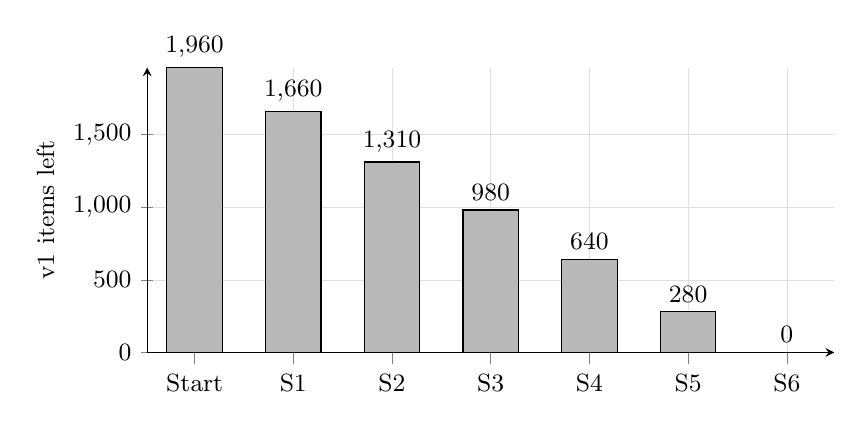
\begin{tikzpicture}
\begin{axis}[halberdplot, ybar, bar width=20pt, width=0.85\textwidth, height=5.2cm, ymin=0, enlarge x limits=0.08, symbolic x coords={Start,S1,S2,S3,S4,S5,S6}, xtick=data, nodes near coords, every node near coord/.append style={font=\figfont}, ylabel={v1 items left}, axis lines*=left, ymajorgrids]
\addplot[fill=gray!55, draw=black, line width=0.4pt] coordinates {(Start,1960) (S1,1660) (S2,1310) (S3,980) (S4,640) (S5,280) (S6,0)};
\end{axis}
\end{tikzpicture}
\caption{The whole v1 list, sprint by sprint.}
\end{figure}
\begin{table}[H]\centering\figfont
\begin{tabular}{@{}c l r r r r r@{}}
\toprule
Sprint & Dates & Committed & Done & Carried & Done \% (X) & Items left \\
\midrule
1 & 10-05 -- 10-16 & 320 & 300 & 20 & 94 & 1,660 \\
2 & 10-19 -- 10-30 & 360 & 350 & 10 & 97 & 1,310 \\
3 & 11-02 -- 11-13 & 375 & 330 & 45 & 88 & 980 \\
4 & 11-16 -- 11-25 & 360 & 340 & 20 & 94 & 640 \\
5 & 11-30 -- 12-11 & 370 & 360 & 10 & 97 & 280 \\
6 & 12-14 -- 12-23 & 280 & 280 & 0 & 100 & 0 \\
\bottomrule
\end{tabular}
\caption{Sprint totals, computed from the compiled journal by \texttt{Scrum::sprint\_summary}; the generator stops if any differs from the doc.}
\end{table}
\section{Funding and earned value}
A notional FY27 funding journal sits beside the stand-up journal, in the same ledger format (\texttt{data/halberd/funding.ledger}). Each segment is budgeted at a notional \$150 per v1 item, time-phased over the days the plan works it. \$323,400 is authorized on 1 October: the budget at completion of \$294,000 plus a 10\% reserve. Labor posts weekly from the items actually ported; sprint 3 overran while it waited on the shared runner. Percent complete comes from the stand-ups, so earned value is computed, not estimated.

\begin{figure}[H]\centering
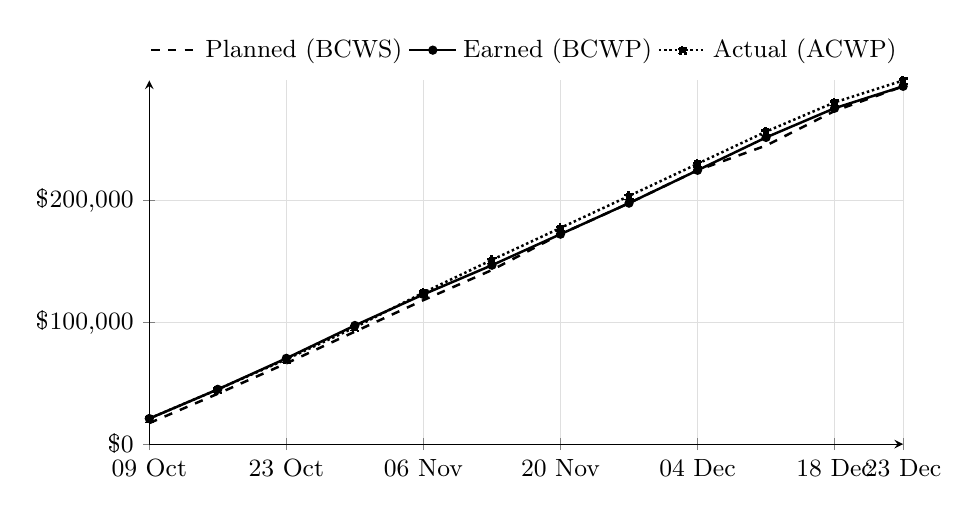
\begin{tikzpicture}
\begin{axis}[halberdplot, width=0.92\textwidth, height=6.2cm, xtick={0,2,4,6,8,10,11}, xticklabels={{09 Oct},{23 Oct},{06 Nov},{20 Nov},{04 Dec},{18 Dec},{23 Dec}}, scaled y ticks=false, yticklabel style={/pgf/number format/.cd, fixed, precision=0, 1000 sep={\mbox{,}}}, ymin=0, yticklabel={\$\pgfmathprintnumber{\tick}}, legend columns=3]
\addplot[black, dashed] coordinates {(0,17250.0) (1,41400.0) (2,66370.2) (3,92434.0) (4,118307.1) (5,143057.1) (6,172500.0) (7,198000.0) (8,225000.0) (9,245333.3) (10,273750.0) (11,294000.0)};
\addlegendentry{Planned (BCWS)}
\addplot[black, mark=*] coordinates {(0,21000.0) (1,45000.0) (2,70500.0) (3,97500.0) (4,123000.0) (5,147000.0) (6,172500.0) (7,198000.0) (8,225000.0) (9,252000.0) (10,276000.0) (11,294000.0)};
\addlegendentry{Earned (BCWP)}
\addplot[black, densely dotted, mark=square*] coordinates {(0,21000.0) (1,45000.0) (2,69735.0) (3,95925.0) (4,124485.0) (5,151365.0) (6,177630.0) (7,203895.0) (8,230355.0) (9,256815.0) (10,280815.0) (11,298815.0)};
\addlegendentry{Actual (ACWP)}
\end{axis}
\end{tikzpicture}
\caption{Cumulative cost at the end of each week.}
\end{figure}
\begin{figure}[H]\centering
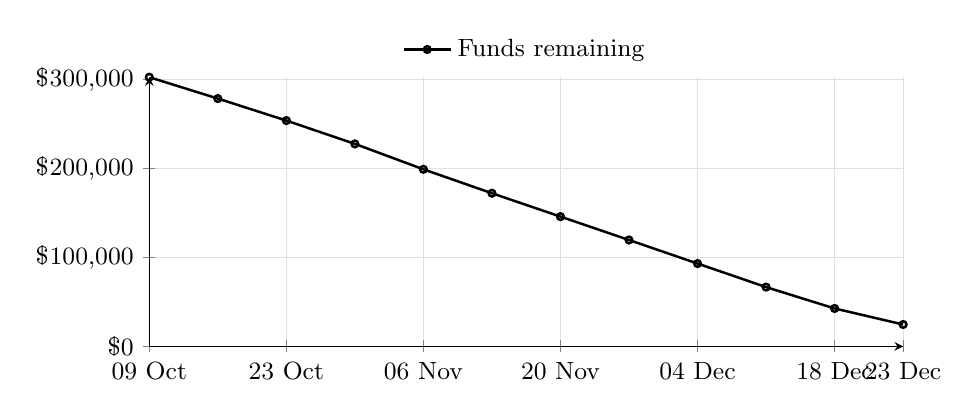
\begin{tikzpicture}
\begin{axis}[halberdplot, width=0.92\textwidth, height=5cm, xtick={0,2,4,6,8,10,11}, xticklabels={{09 Oct},{23 Oct},{06 Nov},{20 Nov},{04 Dec},{18 Dec},{23 Dec}}, scaled y ticks=false, yticklabel style={/pgf/number format/.cd, fixed, precision=0, 1000 sep={\mbox{,}}}, ymin=0, yticklabel={\$\pgfmathprintnumber{\tick}}, legend columns=1]
\addplot[black, mark=o] coordinates {(0,302400.0) (1,278400.0) (2,253665.0) (3,227475.0) (4,198915.0) (5,172035.0) (6,145770.0) (7,119505.0) (8,93045.0) (9,66585.0) (10,42585.0) (11,24585.0)};
\addlegendentry{Funds remaining}
\end{axis}
\end{tikzpicture}
\caption{Funds remaining at the end of each week.}
\end{figure}
\subsection{Earned value at 30 October 2026}
{\figfont\setlength{\tabcolsep}{3pt}
\begin{tabular}{@{}l r r r r r r r r r r@{}}
\toprule
Segment & Done & BAC & BCWS & BCWP & ACWP & CV & SV & CPI & SPI & EAC \\
\midrule
E Systems Engineering \& Integration & 100\% & \$55,200 & \$55,200 & \$55,200 & \$54,894 & \$306 & \$0 & 1.01 & 1.00 & \$54,894 \\
V Interceptor Development & 81\% & \$52,500 & \$37,234 & \$42,300 & \$41,031 & \$1,269 & \$5,066 & 1.03 & 1.14 & \$50,925 \\
B Battle Management \& Fire Control & 0\% & \$49,500 & \$0 & \$0 & \$0 & \$0 & \$0 & -- & -- & -- \\
T Test \& Evaluation & 0\% & \$40,800 & \$0 & \$0 & \$0 & \$0 & \$0 & -- & -- & -- \\
G Government Program Office & 0\% & \$27,000 & \$0 & \$0 & \$0 & \$0 & \$0 & -- & -- & -- \\
M Manufacturing \& Production & 0\% & \$36,600 & \$0 & \$0 & \$0 & \$0 & \$0 & -- & -- & -- \\
L Logistics \& Sustainment & 0\% & \$32,400 & \$0 & \$0 & \$0 & \$0 & \$0 & -- & -- & -- \\
\midrule
\textbf{Total} & 33\% & \$294,000 & \$92,434 & \$97,500 & \$95,925 & \$1,575 & \$5,066 & 1.02 & 1.05 & \$289,251 \\
\bottomrule
\end{tabular}}

\subsection{Earned value at 25 November 2026}
{\figfont\setlength{\tabcolsep}{3pt}
\begin{tabular}{@{}l r r r r r r r r r r@{}}
\toprule
Segment & Done & BAC & BCWS & BCWP & ACWP & CV & SV & CPI & SPI & EAC \\
\midrule
E Systems Engineering \& Integration & 100\% & \$55,200 & \$55,200 & \$55,200 & \$54,894 & \$306 & \$0 & 1.01 & 1.00 & \$54,894 \\
V Interceptor Development & 100\% & \$52,500 & \$52,500 & \$52,500 & \$52,455 & \$45 & \$0 & 1.00 & 1.00 & \$52,455 \\
B Battle Management \& Fire Control & 100\% & \$49,500 & \$49,500 & \$49,500 & \$54,522 & $-$\$5,022 & \$0 & 0.91 & 1.00 & \$54,522 \\
T Test \& Evaluation & 100\% & \$40,800 & \$40,800 & \$40,800 & \$42,024 & $-$\$1,224 & \$0 & 0.97 & 1.00 & \$42,024 \\
G Government Program Office & 0\% & \$27,000 & \$0 & \$0 & \$0 & \$0 & \$0 & -- & -- & -- \\
M Manufacturing \& Production & 0\% & \$36,600 & \$0 & \$0 & \$0 & \$0 & \$0 & -- & -- & -- \\
L Logistics \& Sustainment & 0\% & \$32,400 & \$0 & \$0 & \$0 & \$0 & \$0 & -- & -- & -- \\
\midrule
\textbf{Total} & 67\% & \$294,000 & \$198,000 & \$198,000 & \$203,895 & $-$\$5,895 & \$0 & 0.97 & 1.00 & \$302,753 \\
\bottomrule
\end{tabular}}

Funds remaining \$119,505; average burn over the last two months \$95,925 a month; at that rate the money lasts 1.2 more months (to 2027-01-03).

\subsection{Earned value at 23 December 2026}
{\figfont\setlength{\tabcolsep}{3pt}
\begin{tabular}{@{}l r r r r r r r r r r@{}}
\toprule
Segment & Done & BAC & BCWS & BCWP & ACWP & CV & SV & CPI & SPI & EAC \\
\midrule
E Systems Engineering \& Integration & 100\% & \$55,200 & \$55,200 & \$55,200 & \$54,894 & \$306 & \$0 & 1.01 & 1.00 & \$54,894 \\
V Interceptor Development & 100\% & \$52,500 & \$52,500 & \$52,500 & \$52,455 & \$45 & \$0 & 1.00 & 1.00 & \$52,455 \\
B Battle Management \& Fire Control & 100\% & \$49,500 & \$49,500 & \$49,500 & \$54,522 & $-$\$5,022 & \$0 & 0.91 & 1.00 & \$54,522 \\
T Test \& Evaluation & 100\% & \$40,800 & \$40,800 & \$40,800 & \$42,024 & $-$\$1,224 & \$0 & 0.97 & 1.00 & \$42,024 \\
G Government Program Office & 100\% & \$27,000 & \$27,000 & \$27,000 & \$26,460 & \$540 & \$0 & 1.02 & 1.00 & \$26,460 \\
M Manufacturing \& Production & 100\% & \$36,600 & \$36,600 & \$36,600 & \$36,060 & \$540 & \$0 & 1.01 & 1.00 & \$36,060 \\
L Logistics \& Sustainment & 100\% & \$32,400 & \$32,400 & \$32,400 & \$32,400 & \$0 & \$0 & 1.00 & 1.00 & \$32,400 \\
\midrule
\textbf{Total} & 100\% & \$294,000 & \$294,000 & \$294,000 & \$298,815 & $-$\$4,815 & \$0 & 0.98 & 1.00 & \$298,815 \\
\bottomrule
\end{tabular}}

\textbf{At the finish:} \$298,815 spent against a \$294,000 budget (CPI 0.98); \$24,585 of the \$323,400 authorized is left, so the overrun came out of the reserve.

{\figfont\itshape CPI = earned / actual (above 1 is under cost); SPI = earned / planned (above 1 is ahead); EAC = BAC / CPI. The same numbers come from \texttt{bin/ledger.pl evm} and \texttt{forecast}.\par}
\section{Sprints and daily stand-ups}
Each stand-up answers yesterday, today and blockers, in the alphabet of the A--Z metrics. A dagger\blk{} marks a blocked day.
\clearpage
\subsection{Sprint 1: 5 October 2026 to 16 October 2026}
Committed 320. Done 300. Carried over 20. Done 94\% (X).

\begin{center}
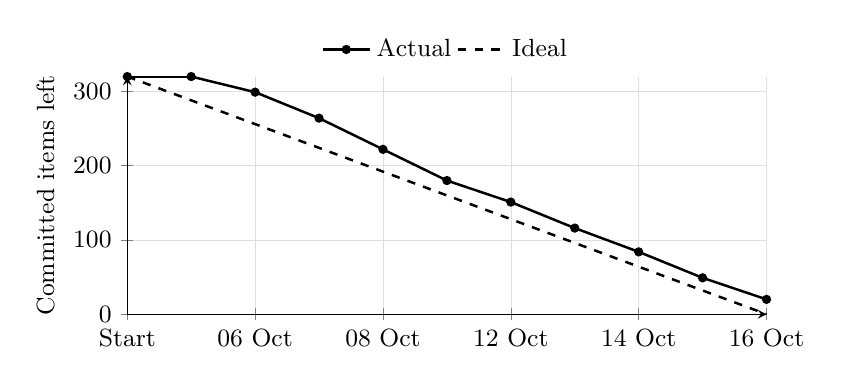
\begin{tikzpicture}
\begin{axis}[halberdplot, width=0.8\textwidth, height=4.6cm, xtick={0,2,4,6,8,10}, xticklabels={{Start},{06 Oct},{08 Oct},{12 Oct},{14 Oct},{16 Oct}}, ylabel={Committed items left}, legend columns=2]
\addplot[black, mark=*] coordinates {(0,320.0) (1,320.0) (2,299.0) (3,264.0) (4,222.0) (5,180.0) (6,151.0) (7,116.0) (8,84.0) (9,49.0) (10,20.0)};
\addlegendentry{Actual}
\addplot[black, dashed] coordinates {(0,320.0) (1,288.0) (2,256.0) (3,224.0) (4,192.0) (5,160.0) (6,128.0) (7,96.0) (8,64.0) (9,32.0) (10,0.0)};
\addlegendentry{Ideal}
\end{axis}
\end{tikzpicture}
\end{center}
{\figfont\setlength{\tabcolsep}{4pt}\renewcommand{\arraystretch}{1.15}
\begin{longtable}{@{}>{\raggedright}p{0.075\textwidth} r r >{\raggedright}p{0.34\textwidth} >{\raggedright}p{0.22\textwidth} >{\raggedright\arraybackslash}p{0.17\textwidth}@{}}
\toprule
Day & Ported & Left & Yesterday & Today & Blockers \\
\midrule
\endhead
\bottomrule
\endfoot
Mon 05 Oct & 0 & 1,960 & Nothing yet; the pipeline goes up today. & Setting up the repo, the pre-commit gate and the CI lint job. & -- \\
Tue 06 Oct & 21 & 1,939 & The pipeline is up: pre-commit gate and CI lint job, 0/0 to merge (E). & Continuing Systems Engineering \& Integration. & -- \\
Wed 07 Oct & 35 & 1,904 & 21 more elements under configuration control, now 1\% (A), all merged at 0/0 (E). & More of Systems Engineering \& Integration goes under configuration control today. & -- \\
Thu 08 Oct & 42 & 1,862 & 35 more elements under configuration control, now 3\% (A), all merged at 0/0 (E). & Bringing more of Systems Engineering \& Integration under the pipeline. & -- \\
Fri 09 Oct & 42 & 1,820 & 42 more elements under configuration control, now 5\% (A), all merged at 0/0 (E). & Continuing Systems Engineering \& Integration. & -- \\
Mon 12 Oct & 29 & 1,791 & 42 more elements under configuration control, now 7\% (A), all merged at 0/0 (E). & Importing the first DOORS module. & -- \\
Tue 13 Oct & 35 & 1,756 & 29 more elements under configuration control, now 9\% (A), all merged at 0/0 (E). The first DOORS module is in, and requirements are now linking to model elements (C). 2 orphan and 4 unverified requirements, flagged to owners (F, G). & Bringing more of Systems Engineering \& Integration under the pipeline. & -- \\
Wed 14 Oct & 32 & 1,724 & 35 more elements under configuration control, now 10\% (A), all merged at 0/0 (E). 1 of 2 zone-crossing interfaces still need a security requirement (Q). & Continuing Systems Engineering \& Integration. & -- \\
Thu 15 Oct & 35 & 1,689 & 32 more elements under configuration control, now 12\% (A), all merged at 0/0 (E). 54 of 1,450 DOORS requirements linked (C). & More of Systems Engineering \& Integration goes under configuration control today. & -- \\
Fri 16 Oct & 29 & 1,660 & 35 more elements under configuration control, now 14\% (A), all merged at 0/0 (E). 3 interface mismatches caught at merge to date, 0 reached integration (H). & Bringing more of Systems Engineering \& Integration under the pipeline. & -- \\
\end{longtable}}
\clearpage
\subsection{Sprint 2: 19 October 2026 to 30 October 2026}
Committed 360. Done 350. Carried over 10. Done 97\% (X). Includes HAL-10, 20 items carried in from sprint 1.

\begin{center}
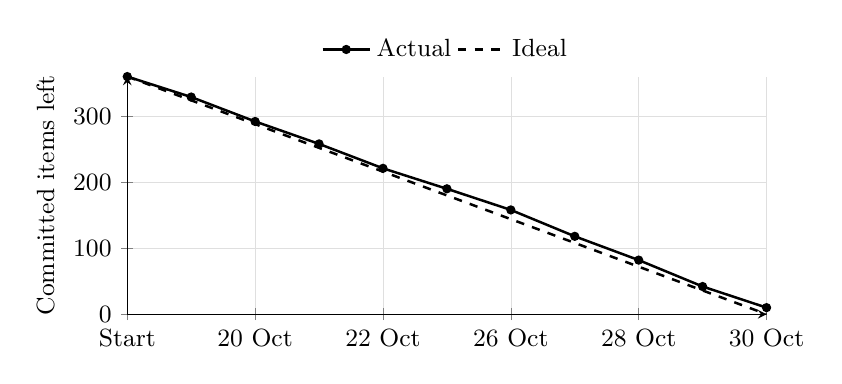
\begin{tikzpicture}
\begin{axis}[halberdplot, width=0.8\textwidth, height=4.6cm, xtick={0,2,4,6,8,10}, xticklabels={{Start},{20 Oct},{22 Oct},{26 Oct},{28 Oct},{30 Oct}}, ylabel={Committed items left}, legend columns=2]
\addplot[black, mark=*] coordinates {(0,360.0) (1,329.0) (2,292.0) (3,258.0) (4,221.0) (5,190.0) (6,158.0) (7,118.0) (8,82.0) (9,42.0) (10,10.0)};
\addlegendentry{Actual}
\addplot[black, dashed] coordinates {(0,360.0) (1,324.0) (2,288.0) (3,252.0) (4,216.0) (5,180.0) (6,144.0) (7,108.0) (8,72.0) (9,36.0) (10,0.0)};
\addlegendentry{Ideal}
\end{axis}
\end{tikzpicture}
\end{center}
{\figfont\setlength{\tabcolsep}{4pt}\renewcommand{\arraystretch}{1.15}
\begin{longtable}{@{}>{\raggedright}p{0.075\textwidth} r r >{\raggedright}p{0.34\textwidth} >{\raggedright}p{0.22\textwidth} >{\raggedright\arraybackslash}p{0.17\textwidth}@{}}
\toprule
Day & Ported & Left & Yesterday & Today & Blockers \\
\midrule
\endhead
\bottomrule
\endfoot
Mon 19 Oct & 31 & 1,629 & 29 more elements under configuration control, now 15\% (A), all merged at 0/0 (E). 12 orphan and 20 unverified requirements, flagged to owners (F, G). & Continuing Systems Engineering \& Integration. & -- \\
Tue 20 Oct & 37 & 1,592 & 31 more elements under configuration control, now 17\% (A), all merged at 0/0 (E). 2 of 5 zone-crossing interfaces still need a security requirement (Q). & Finishing Systems Engineering \& Integration; it should be gated by end of day. & -- \\
Wed 21 Oct & 34 & 1,558 & 37 more elements under configuration control, now 19\% (A), all merged at 0/0 (E). Systems Engineering \& Integration is now gated on every merge: 1 of 7 segments (B). 138 of 1,450 DOORS requirements linked (C). & Bringing more of Interceptor Development under the pipeline. & -- \\
Thu 22 Oct & 37 & 1,521 & 34 more elements under configuration control, now 21\% (A), all merged at 0/0 (E). 8 interface mismatches caught at merge to date, 0 reached integration (H). & Continuing Interceptor Development. & -- \\
Fri 23 Oct & 31 & 1,490 & 37 more elements under configuration control, now 22\% (A), all merged at 0/0 (E). 36 orphan and 49 unverified requirements, flagged to owners (F, G). & More of Interceptor Development goes under configuration control today. & -- \\
Mon 26 Oct & 32 & 1,458 & 31 more elements under configuration control, now 24\% (A), all merged at 0/0 (E). 3 of 7 zone-crossing interfaces still need a security requirement (Q). & Bringing more of Interceptor Development under the pipeline. & -- \\
Tue 27 Oct & 40 & 1,418 & 32 more elements under configuration control, now 26\% (A), all merged at 0/0 (E). 233 of 1,450 DOORS requirements linked (C). & Continuing Interceptor Development. & -- \\
Wed 28 Oct & 36 & 1,382 & 40 more elements under configuration control, now 28\% (A), all merged at 0/0 (E). 13 interface mismatches caught at merge to date, 0 reached integration (H). & More of Interceptor Development goes under configuration control today. & -- \\
Thu 29 Oct & 40 & 1,342 & 36 more elements under configuration control, now 29\% (A), all merged at 0/0 (E). 56 orphan and 70 unverified requirements, flagged to owners (F, G). & Generating the interface table from the model. & -- \\
Fri 30 Oct & 32 & 1,310 & 40 more elements under configuration control, now 32\% (A), all merged at 0/0 (E). The interface table is now generated from the model: 1 of 12 program documents (L), 0 hand edits (M). 2 of 9 zone-crossing interfaces still need a security requirement (Q). & Tagging baseline 1. & -- \\
\end{longtable}}
\clearpage
\subsection{Sprint 3: 2 November 2026 to 13 November 2026}
Committed 375. Done 330. Carried over 45. Done 88\% (X). Includes HAL-21, 10 items carried in from sprint 2.

\begin{center}
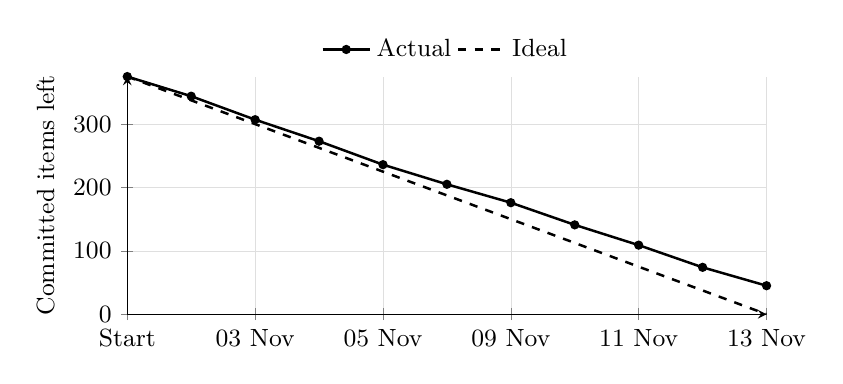
\begin{tikzpicture}
\begin{axis}[halberdplot, width=0.8\textwidth, height=4.6cm, xtick={0,2,4,6,8,10}, xticklabels={{Start},{03 Nov},{05 Nov},{09 Nov},{11 Nov},{13 Nov}}, ylabel={Committed items left}, legend columns=2]
\addplot[black, mark=*] coordinates {(0,375.0) (1,344.0) (2,307.0) (3,273.0) (4,236.0) (5,205.0) (6,176.0) (7,141.0) (8,109.0) (9,74.0) (10,45.0)};
\addlegendentry{Actual}
\addplot[black, dashed] coordinates {(0,375.0) (1,337.5) (2,300.0) (3,262.5) (4,225.0) (5,187.5) (6,150.0) (7,112.5) (8,75.0) (9,37.5) (10,0.0)};
\addlegendentry{Ideal}
\end{axis}
\end{tikzpicture}
\end{center}
{\figfont\setlength{\tabcolsep}{4pt}\renewcommand{\arraystretch}{1.15}
\begin{longtable}{@{}>{\raggedright}p{0.075\textwidth} r r >{\raggedright}p{0.34\textwidth} >{\raggedright}p{0.22\textwidth} >{\raggedright\arraybackslash}p{0.17\textwidth}@{}}
\toprule
Day & Ported & Left & Yesterday & Today & Blockers \\
\midrule
\endhead
\bottomrule
\endfoot
Mon 02 Nov & 31 & 1,279 & 32 more elements under configuration control, now 33\% (A), all merged at 0/0 (E). Baseline 1 is tagged: 650 elements (D), and it rebuilds identically (S). 340 of 1,450 DOORS requirements linked (C). & More of Interceptor Development goes under configuration control today. & -- \\
Tue 03 Nov & 37 & 1,242 & 31 more elements under configuration control, now 35\% (A), all merged at 0/0 (E). 18 interface mismatches caught at merge to date, 0 reached integration (H). & Finishing Interceptor Development; it should be gated by end of day. & -- \\
Wed 04 Nov\blk & 34 & 1,208 & 37 more elements under configuration control, now 37\% (A), all merged at 0/0 (E). Interceptor Development is now gated on every merge: 2 of 7 segments (B). 63 orphan and 78 unverified requirements, flagged to owners (F, G). & Continuing Battle Management \& Fire Control. & Waiting on a shared runner. Gating locally with the pre-commit hook meanwhile (Y). \\
Thu 05 Nov\blk & 37 & 1,171 & 34 more elements under configuration control, now 38\% (A), all merged at 0/0 (E). & More of Battle Management \& Fire Control goes under configuration control today. & Still waiting on the shared runner (Y). \\
Fri 06 Nov\blk & 31 & 1,140 & 37 more elements under configuration control, now 40\% (A), all merged at 0/0 (E). 454 of 1,450 DOORS requirements linked (C). & Bringing more of Battle Management \& Fire Control under the pipeline. & Runner still pending; asked for it again (Y). \\
Mon 09 Nov & 29 & 1,111 & 31 more elements under configuration control, now 42\% (A), all merged at 0/0 (E). 25 interface mismatches caught at merge to date, 0 reached integration (H). The shared runner is live. & Continuing Battle Management \& Fire Control. & -- \\
Tue 10 Nov & 35 & 1,076 & 29 more elements under configuration control, now 43\% (A), all merged at 0/0 (E). 56 orphan and 72 unverified requirements, flagged to owners (F, G). & More of Battle Management \& Fire Control goes under configuration control today. & -- \\
Wed 11 Nov & 32 & 1,044 & 35 more elements under configuration control, now 45\% (A), all merged at 0/0 (E). 3 of 14 zone-crossing interfaces still need a security requirement (Q). & Generating the first ICD view and diffing it against the legacy ICD. & -- \\
Thu 12 Nov & 35 & 1,009 & 32 more elements under configuration control, now 47\% (A), all merged at 0/0 (E). Drift checks found 47 discrepancies in the legacy ICDs, flagged for correction (T). 558 of 1,450 DOORS requirements linked (C). & Continuing Battle Management \& Fire Control. & -- \\
Fri 13 Nov & 29 & 980 & 35 more elements under configuration control, now 49\% (A), all merged at 0/0 (E). 30 interface mismatches caught at merge to date, 0 reached integration (H). & More of Battle Management \& Fire Control goes under configuration control today. & -- \\
\end{longtable}}
\clearpage
\subsection{Sprint 4: 16 November 2026 to 25 November 2026}
Committed 360. Done 340. Carried over 20. Done 94\% (X). Includes HAL-32, 45 items carried in from sprint 3.

\begin{center}
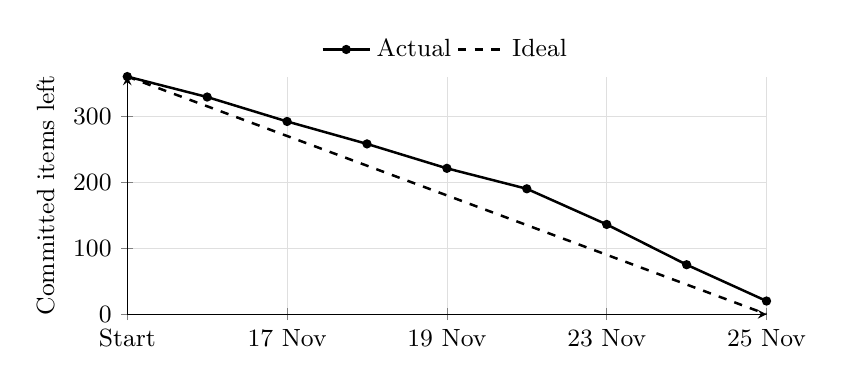
\begin{tikzpicture}
\begin{axis}[halberdplot, width=0.8\textwidth, height=4.6cm, xtick={0,2,4,6,8}, xticklabels={{Start},{17 Nov},{19 Nov},{23 Nov},{25 Nov}}, ylabel={Committed items left}, legend columns=2]
\addplot[black, mark=*] coordinates {(0,360.0) (1,329.0) (2,292.0) (3,258.0) (4,221.0) (5,190.0) (6,136.0) (7,75.0) (8,20.0)};
\addlegendentry{Actual}
\addplot[black, dashed] coordinates {(0,360.0) (1,315.0) (2,270.0) (3,225.0) (4,180.0) (5,135.0) (6,90.0) (7,45.0) (8,0.0)};
\addlegendentry{Ideal}
\end{axis}
\end{tikzpicture}
\end{center}
{\figfont\setlength{\tabcolsep}{4pt}\renewcommand{\arraystretch}{1.15}
\begin{longtable}{@{}>{\raggedright}p{0.075\textwidth} r r >{\raggedright}p{0.34\textwidth} >{\raggedright}p{0.22\textwidth} >{\raggedright\arraybackslash}p{0.17\textwidth}@{}}
\toprule
Day & Ported & Left & Yesterday & Today & Blockers \\
\midrule
\endhead
\bottomrule
\endfoot
Mon 16 Nov & 31 & 949 & 29 more elements under configuration control, now 50\% (A), all merged at 0/0 (E). 47 orphan and 63 unverified requirements, flagged to owners (F, G). & Bringing more of Battle Management \& Fire Control under the pipeline. & -- \\
Tue 17 Nov & 37 & 912 & 31 more elements under configuration control, now 52\% (A), all merged at 0/0 (E). 1 of 16 zone-crossing interfaces still need a security requirement (Q). & Finishing Battle Management \& Fire Control; it should be gated by end of day. & -- \\
Wed 18 Nov & 34 & 878 & 37 more elements under configuration control, now 53\% (A), all merged at 0/0 (E). Battle Management \& Fire Control is now gated on every merge: 3 of 7 segments (B). 3 of 7 segment owners now merge their own changes (Z). 670 of 1,450 DOORS requirements linked (C). & More of Test \& Evaluation goes under configuration control today. & -- \\
Thu 19 Nov & 37 & 841 & 34 more elements under configuration control, now 55\% (A), all merged at 0/0 (E). 36 interface mismatches caught at merge to date, 0 reached integration (H). & Bringing more of Test \& Evaluation under the pipeline. & -- \\
Fri 20 Nov & 31 & 810 & 37 more elements under configuration control, now 57\% (A), all merged at 0/0 (E). 51 orphan and 61 unverified requirements, flagged to owners (F, G). & Continuing Test \& Evaluation. & -- \\
Mon 23 Nov & 54 & 756 & 31 more elements under configuration control, now 59\% (A), all merged at 0/0 (E). 3 of 19 zone-crossing interfaces still need a security requirement (Q). & More of Test \& Evaluation goes under configuration control today. & -- \\
Tue 24 Nov & 61 & 695 & 54 more elements under configuration control, now 61\% (A), all merged at 0/0 (E). 804 of 1,450 DOORS requirements linked (C). & Wiring the T2 pre-flight prediction inputs to the model. & -- \\
Wed 25 Nov & 55 & 640 & 61 more elements under configuration control, now 65\% (A), all merged at 0/0 (E). 64 of 64 pre-flight prediction parameters now come from the model (O), and 12 of 12 prediction runs name their baseline (P). 41 interface mismatches caught at merge to date, 0 reached integration (H). & Tagging baseline 2 before the holiday. & -- \\
\end{longtable}}
\clearpage
\subsection{Sprint 5: 30 November 2026 to 11 December 2026}
Committed 370. Done 360. Carried over 10. Done 97\% (X). Includes HAL-40, 20 items carried in from sprint 4.

\begin{center}
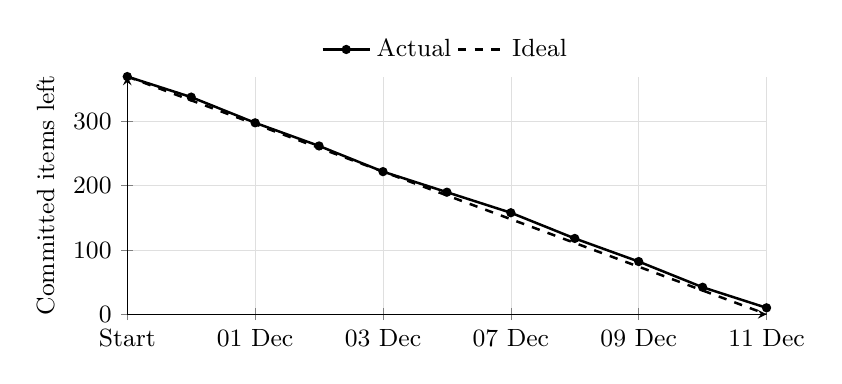
\begin{tikzpicture}
\begin{axis}[halberdplot, width=0.8\textwidth, height=4.6cm, xtick={0,2,4,6,8,10}, xticklabels={{Start},{01 Dec},{03 Dec},{07 Dec},{09 Dec},{11 Dec}}, ylabel={Committed items left}, legend columns=2]
\addplot[black, mark=*] coordinates {(0,370.0) (1,338.0) (2,298.0) (3,262.0) (4,222.0) (5,190.0) (6,158.0) (7,118.0) (8,82.0) (9,42.0) (10,10.0)};
\addlegendentry{Actual}
\addplot[black, dashed] coordinates {(0,370.0) (1,333.0) (2,296.0) (3,259.0) (4,222.0) (5,185.0) (6,148.0) (7,111.0) (8,74.0) (9,37.0) (10,0.0)};
\addlegendentry{Ideal}
\end{axis}
\end{tikzpicture}
\end{center}
{\figfont\setlength{\tabcolsep}{4pt}\renewcommand{\arraystretch}{1.15}
\begin{longtable}{@{}>{\raggedright}p{0.075\textwidth} r r >{\raggedright}p{0.34\textwidth} >{\raggedright}p{0.22\textwidth} >{\raggedright\arraybackslash}p{0.17\textwidth}@{}}
\toprule
Day & Ported & Left & Yesterday & Today & Blockers \\
\midrule
\endhead
\bottomrule
\endfoot
Mon 30 Nov & 32 & 608 & 55 more elements under configuration control, now 67\% (A), all merged at 0/0 (E). Test \& Evaluation is now gated on every merge: 4 of 7 segments (B). 4 of 7 segment owners now merge their own changes (Z). Baseline 2 is tagged: 1,320 elements (D), rebuilds identically (S). 39 orphan and 48 unverified requirements, flagged to owners (F, G). & More of Government Program Office goes under configuration control today. & -- \\
Tue 01 Dec & 40 & 568 & 32 more elements under configuration control, now 69\% (A), all merged at 0/0 (E). & Bringing more of Government Program Office under the pipeline. & -- \\
Wed 02 Dec & 36 & 532 & 40 more elements under configuration control, now 71\% (A), all merged at 0/0 (E). 960 of 1,450 DOORS requirements linked (C). & Continuing Government Program Office. & -- \\
Thu 03 Dec & 40 & 492 & 36 more elements under configuration control, now 73\% (A), all merged at 0/0 (E). & Reviewing threat and mitigation coverage with the ISSM. & -- \\
Fri 04 Dec & 32 & 460 & 40 more elements under configuration control, now 75\% (A), all merged at 0/0 (E). 2 of 12 recorded threats lack a traced mitigation (R). 30 orphan and 37 unverified requirements, flagged to owners (F, G). & Measuring lead time on the last 10 merges. & -- \\
Mon 07 Dec & 32 & 428 & 32 more elements under configuration control, now 77\% (A), all merged at 0/0 (E). Government Program Office is now gated on every merge: 5 of 7 segments (B). 5 of 7 segment owners now merge their own changes (Z). A model change now reaches a reviewed baseline in 4 days; the old change board cycle took 19 (N). & Continuing Manufacturing \& Production. & -- \\
Tue 08 Dec & 40 & 388 & 32 more elements under configuration control, now 78\% (A), all merged at 0/0 (E). 1,078 of 1,450 DOORS requirements linked (C). & More of Manufacturing \& Production goes under configuration control today. & -- \\
Wed 09 Dec & 36 & 352 & 40 more elements under configuration control, now 80\% (A), all merged at 0/0 (E). 47 interface mismatches caught at merge to date, 0 reached integration (H). & Generating the remaining ICD views. & -- \\
Thu 10 Dec & 40 & 312 & 36 more elements under configuration control, now 82\% (A), all merged at 0/0 (E). 8 of 12 program documents now come straight from the model (L), about 30 labor hours saved per baseline (J). 21 orphan and 27 unverified requirements, flagged to owners (F, G). & Continuing Manufacturing \& Production. & -- \\
Fri 11 Dec & 32 & 280 & 40 more elements under configuration control, now 84\% (A), all merged at 0/0 (E). 0 of 25 zone-crossing interfaces still need a security requirement (Q). & More of Manufacturing \& Production goes under configuration control today. & -- \\
\end{longtable}}
\clearpage
\subsection{Sprint 6: 14 December 2026 to 23 December 2026}
Committed 280. Done 280. Carried over 0. Done 100\% (X). Includes HAL-51, 10 items carried in from sprint 5.

\begin{center}
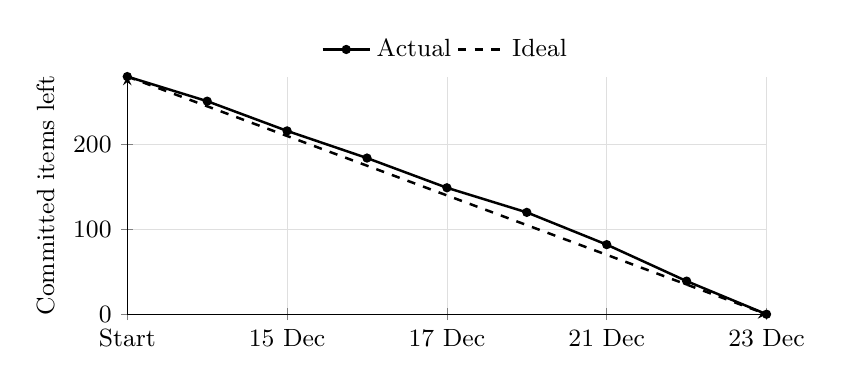
\begin{tikzpicture}
\begin{axis}[halberdplot, width=0.8\textwidth, height=4.6cm, xtick={0,2,4,6,8}, xticklabels={{Start},{15 Dec},{17 Dec},{21 Dec},{23 Dec}}, ylabel={Committed items left}, legend columns=2]
\addplot[black, mark=*] coordinates {(0,280.0) (1,251.0) (2,216.0) (3,184.0) (4,149.0) (5,120.0) (6,82.0) (7,39.0) (8,0.0)};
\addlegendentry{Actual}
\addplot[black, dashed] coordinates {(0,280.0) (1,245.0) (2,210.0) (3,175.0) (4,140.0) (5,105.0) (6,70.0) (7,35.0) (8,0.0)};
\addlegendentry{Ideal}
\end{axis}
\end{tikzpicture}
\end{center}
{\figfont\setlength{\tabcolsep}{4pt}\renewcommand{\arraystretch}{1.15}
\begin{longtable}{@{}>{\raggedright}p{0.075\textwidth} r r >{\raggedright}p{0.34\textwidth} >{\raggedright}p{0.22\textwidth} >{\raggedright\arraybackslash}p{0.17\textwidth}@{}}
\toprule
Day & Ported & Left & Yesterday & Today & Blockers \\
\midrule
\endhead
\bottomrule
\endfoot
Mon 14 Dec & 29 & 251 & 32 more elements under configuration control, now 86\% (A), all merged at 0/0 (E). 1,210 of 1,450 DOORS requirements linked (C). & Bringing more of Manufacturing \& Production under the pipeline. & -- \\
Tue 15 Dec & 35 & 216 & 29 more elements under configuration control, now 87\% (A), all merged at 0/0 (E). & Finishing Manufacturing \& Production; it should be gated by end of day. & -- \\
Wed 16 Dec & 32 & 184 & 35 more elements under configuration control, now 89\% (A), all merged at 0/0 (E). Manufacturing \& Production is now gated on every merge: 6 of 7 segments (B). 6 of 7 segment owners now merge their own changes (Z). 13 orphan and 18 unverified requirements, flagged to owners (F, G). & Rebuilding the gate after this morning's parser update. & -- \\
Thu 17 Dec & 35 & 149 & 32 more elements under configuration control, now 91\% (A), all merged at 0/0 (E). The gate broke on a parser update and was restored in 2 hours (W). ICD views regenerate in 6 minutes (K). & Bringing more of Logistics \& Sustainment under the pipeline. & -- \\
Fri 18 Dec & 29 & 120 & 35 more elements under configuration control, now 92\% (A), all merged at 0/0 (E). 1,333 of 1,450 DOORS requirements linked (C). & Continuing Logistics \& Sustainment. & -- \\
Mon 21 Dec & 38 & 82 & 29 more elements under configuration control, now 94\% (A), all merged at 0/0 (E). & More of Logistics \& Sustainment goes under configuration control today. & -- \\
Tue 22 Dec & 43 & 39 & 38 more elements under configuration control, now 96\% (A), all merged at 0/0 (E). 6 orphan and 9 unverified requirements, flagged to owners (F, G). & Bringing more of Logistics \& Sustainment under the pipeline. & -- \\
Wed 23 Dec & 39 & 0 & 43 more elements under configuration control, now 98\% (A), all merged at 0/0 (E). & Tagging baseline 3. & -- \\
\end{longtable}}
\end{document}
